\chapter{Konfigurasi dan Hasil Timing Diagram dari Verilator}
\label{appendix:verilator}

Terdapat dua unit pengujian yang dilakukan untuk mengetahui akurasi yang dimiliki oleh akselerator: q.max dan q.update. Instruksi lain, digunakan dan diuji sekaligus untuk menguji kedua instruksi tersebut.

Pertama, pengujian q.max, dilakukan dengan membuat sebuah program pada bahasa C pada kode \ref{fig:verilator-qmax}.

\begin{figure}[H]
	\centering
	\begin{lstlisting}[language=C,escapechar=|,numbers=left,caption={Program bahasa C untuk pengujian q.max},label={fig:verilator-qmax},captionpos=b]
int main() {
  setAMax(4);
  storeQValue(10.2, 0);
  storeQValue(6.2, 1);
  storeQValue(3.2, 2);
  storeQValue(12.0, 3);
  getMax(0);
}
\end{lstlisting}
\end{figure}

Hasil dari program diatas, seharusnya menghasilkan indeks 3 sebagai jawaban dari fungsi getMax yang merupakan \ac{BSP} dari q.max. Berikut merupakan hasil sintesis \textit{timing diagram} untuk program \ref{fig:verilator-qmax}.

\begin{figure}[h]
	\centering
	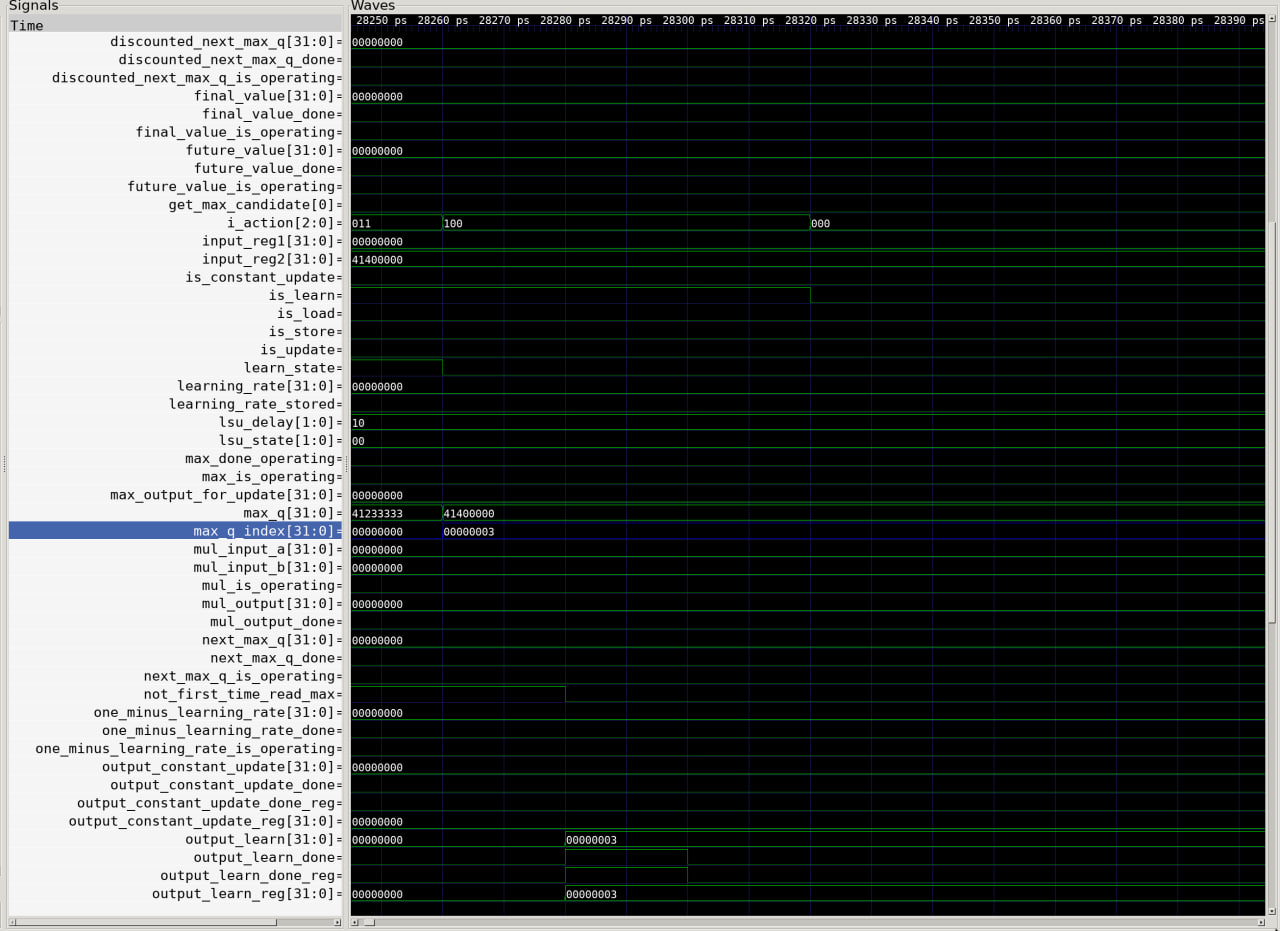
\includegraphics[width=1\textwidth]{appendix/gtkwave-qmax.jpg}
	\caption{Hasil \textit{timing diagram} program q.max}
	\label{fig:gtkwave-qmax}
\end{figure}

Dapat diperhatikan pada gambar \ref{fig:gtkwave-qmax}, bahwa nilai keluaran \textit{max\_q\_index} yang merupakan representasi $a_{max}$ itu bernilai 3. Maka, hasil dari akselerator sudah sesuai untuk instruksi q.max.

Selanjutnya, untuk instruksi q.update, berikut merupakan program yang digunakan untuk menguji akurasi akselerator.


\begin{figure}[H]
	\centering
	\begin{lstlisting}[language=C,escapechar=|,numbers=left,caption={Program bahasa C untuk pengujian q.update},label={fig:verilator-qupdate},captionpos=b]
int main() {
  setAMax(4);
  setConstant(CONSTANT_TYPE_LEARNING_RATE, 0.4);
  setConstant(CONSTANT_TYPE_DISCOUNT_FACTOR, 0.28);
  storeQValue(10.2, 0);
  storeQValue(6.2, 1);
  storeQValue(3.2, 6);
  storeQValue(12.0, 12);
  setNextState(1);
  qUpdate(0, 2.5);
}
\end{lstlisting}
\end{figure}

Bila menggunakan persamaan \ref{eq:q-learning}, maka didapat nilai hasil dari kode \ref{fig:verilator-qupdate} adalah 8.26. Nilai tersebut, bila diubah ke heksadesimal maka akan bernilai 0x410432cb. Program \ref{fig:verilator-qupdate} kemudian dicoba dan didapatkan hasil pada gambar \ref{fig:gtkwave-qupdate}.

\begin{figure}[h]
	\centering
	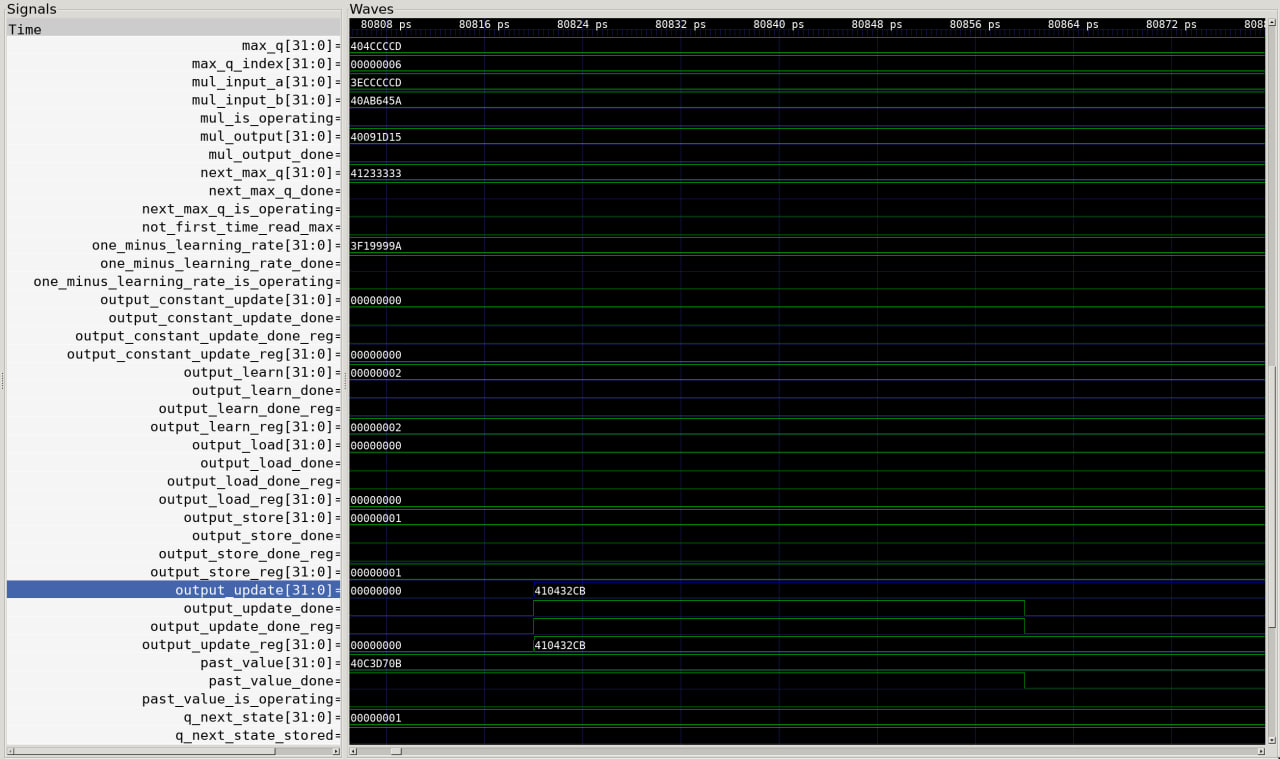
\includegraphics[width=1\textwidth]{appendix/gtkwave-qupdate.jpg}
	\caption{Hasil \textit{timing diagram} program q.update}
	\label{fig:gtkwave-qupdate}
\end{figure}

Dapat dilihat, pada gambar \ref{fig:gtkwave-qupdate}, didapat hasil pada \textit{register} \textit{output update} yang bernilai 0x410432cb. Sehingga, akselerator sudah terimplementasikan secara akurat.
